\subsection{Technical Internals}
{
\tikzset{external/figure name/.add={}{techinternals_}}%

This section describes keys which are usually set by internal routines -- it is typically unnecessary to use them. However, they may impose limitations or influence performance. Such cases are documented clearly in other sections of this manual. This here is the reference on the involved internals.

\begin{pgfplotskey}{cell picture=\mchoice{true,false,if necessary} (initially true)}
	This key is set automatically by \PGFPlots\ if necessary (for example by |set layers|).

	Typically, \PGFPlots\ creates a so-called ``cell picture''. A cell picture is a separate picture which is typeset into a node. Finally, the node is shifted to fulfill special |anchor| requirements. The necessity for a cell picture is given if the |anchor| of an axis is only known after the complete axis has been drawn.

	The initial choice \declaretext{true} means that \PGFPlots\ will create a cell picture for every axis. This allows all |anchor|s, but it is unsuited if multiple graphics layers are desired or if one wants SVG export. In order to create a cell picture, \PGFPlots\ interrupts the embedding |tikzpicture|, draws a new |tikzpicture|, and finally typesets the result into a node.

	The choice \declaretext{false} tells \PGFPlots\ to draw its paths directly into the embedding |tikzpicture|. Such an approach is necessary if the axis shall use layers of the embedding |tikzpicture|. This is possible if and only if the |anchor| can be determined without actually drawing the complete axis. If so, \PGFPlots\ will modify the transformation matrix in advance. Note that axes with |cell picture=false| will \emph{contain} all the usual anchors -- the only difference is that the axis itsself can only use one of the following anchors for its alignment: |north|, |north west|, |west|, |south west|, |south|, |south east|, |east|, |north east|, |north|, |center|, |origin|, |above origin|, |left of origin|, |right of origin|, |below origin|.

	The choice \declaretext{if necessary} will check if the chosen anchor is one of the list above. If so, it will use |cell picture=false|. Otherwise, it will use |cell picture=true|.

\end{pgfplotskey}

\begin{pgfplotskey}{clip mode=\mchoice{global,individual} (initially global)}
	This key controls how \PGFPlots\ implements the |clip=true| feature (which is on by default). Its primary motivation is control where markers are placed: are markers on top of everything else (choice |global|) or are they overdrawn by following plots (choice |individual|)?
	

	The choice \declaretext{global} tells \PGFPlots\ to install one single clip path for the complete picture\footnote{The choice \texttt{clip mode=global} was the only supported clipping mechanism up to and including version 1.5.}.
	In order to avoid clipped marker paths, any markers are processed after the clip path has been closed, i.e.\ on a separate layer (see |clip marker paths|). An unexpected side--effect is that marks are on top of plots, even if the plots have been added after the markers.

	The choice \declaretext{individual} instructs \PGFPlots\ to install a separate clip path for \emph{every} |\addplot| command. Consequently, the plot will be clipped. But most importantly, its markers will be drawn immediately after the clip path has been deactivated.

	An unexpected side--effect of |clip mode=individual| is that 
	\begin{enumerate}
		\item the resulting pdf will be slightly larger due to the repeated paths,
		\item custom drawing instruction like |\node| or |\draw| need to be clipped \emph{manually}: use
\begin{codeexample}[]
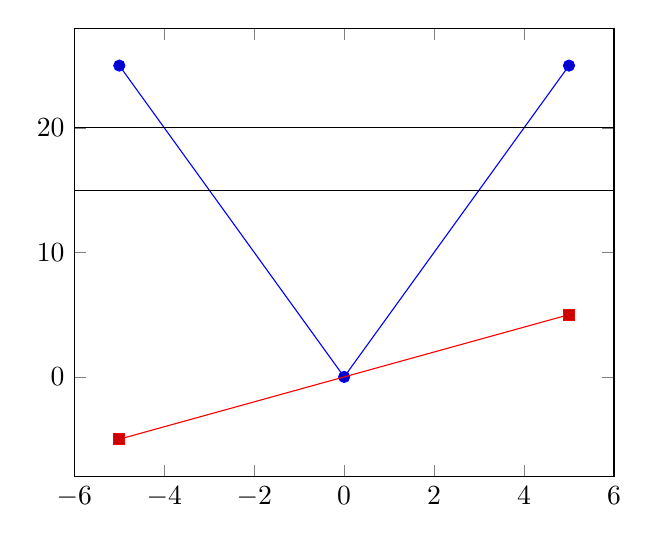
\begin{tikzpicture}
	\begin{axis}[
		clip mode=individual,
	]
	\addplot+[samples=3] {x^2};

	\begin{scope}
		\clip \pgfextra{\pgfplotspathaxisoutline};

		\draw (axis cs:-20,15) -- (axis cs:20,15);

		\draw (axis cs:-20,20) -- (axis cs:20,20);
	\end{scope}

	\addplot+[samples=2] {x};
	\end{axis}
\end{tikzpicture}
\end{codeexample}
		\noindent to install a custom clip path around your |\draw| instructions for such a use--case. Here, the path instruction |\pgfplotspathaxisoutline| results in a path of the axis outline, i.e.\ the path which is used for the background paths or for clipping. Since it is a basic level macro, it needs to be encapsulated by |\pgfextra|.
	\end{enumerate}

	Note that |clip marker paths| can lead to the same result as |clip mode=individual| if the plot does not reach the boundaries.
\end{pgfplotskey}

\begin{pgfplotskey}{compat/show suggested version=\mchoice{true,false} (initially true)}
	If enabled, \PGFPlots\ will show you which value for |compat=|\meta{version} results in the largest active feature set and highest quality.
	
	This key will generate a warning if the current version is so old that the quality degrades seriously.

	The notification will be printed to your |.log| file (during |\end{document}|).
\end{pgfplotskey}
}

